% ----------------------------------------------------------------------
%  Set the document class
% ----------------------------------------------------------------------
\documentclass[11pt,a4paper]{article}
\usepackage[lmargin=2cm, tmargin=3cm, rmargin=2cm, bmargin=2cm, headheight=5cm]{geometry}

% ----------------------------------------------------------------------
% Define external packages, language, margins, fonts and new commands
% ----------------------------------------------------------------------
%\input{preamble} 
\usepackage[utf8]{inputenc}   % <<<<< Linux
\usepackage[english]{babel} % <<<<< English
\usepackage{notoccite}
\usepackage[skip=0.5\baselineskip]{caption}
\hyphenation{GTKWave}
\usepackage{listings}
\usepackage[all]{nowidow}
\usepackage{graphicx}
\usepackage[numbers,sort&compress]{natbib} % <<<<< References in numbered list [1],[2],...
\usepackage{subcaption} 
\usepackage{mdframed}
\usepackage{fancyhdr}
\usepackage{float}
\usepackage{mathtools}
\usepackage{hyperref}
\hypersetup{
    colorlinks,
    citecolor=black,
    filecolor=black,
    linkcolor=black,
    urlcolor=black
}

%\usepackage{setspace}
\renewcommand{\baselinestretch}{1.5}

%Header
\pagestyle{fancy}{
\fancyhf{}
\rhead{
\includegraphics[width=30mm]{Images/IST_A_CMYK_POS.pdf}}
\lhead{Group 67}

%footer
\lfoot{Lisbon, March 22, 2021}
\rfoot{Page \thepage}
}


%%%%%%%%%%%%%%%%%%%%%%%%%%%%%%%%%%%%%%%%%%%%%%%%%%%%%%%%%%%%%%%%%%%%%%%%
%     Begin Document                                                   %
%%%%%%%%%%%%%%%%%%%%%%%%%%%%%%%%%%%%%%%%%%%%%%%%%%%%%%%%%%%%%%%%%%%%%%%%


\begin{document}

\setcounter{page}{0}

% Set roman numbering (i,ii,...) before the start of chapters
%\pagenumbering{roman}

% ----------------------------------------------------------------------
%  Cover page
% ----------------------------------------------------------------------
\thispagestyle {empty}{

% IST Logo - Signature A
% parameters: bb=llx lly urx ury (bounding box), width=h_length, height=v_length, angle=angle, scale=factor, clip=true/false, draft=true/false. 

\includegraphics[bb=9.5cm 11cm 0cm 0cm,scale=0.29]{../../figlib/IST_A_CMYK_POS.pdf}

\begin{center}
%
% Figure (Image or plot)
%\vspace{1.0cm}
% height = 50 mm
%\includegraphics[height=50mm]{Figures/Airbus_A350.jpg}

% Title, author and degree
\textsc{\Large{Audio Amplifier Circuit}}\\[0.5cm] % <<<<< EDIT TITLE
\vspace{0.6cm}
\textsc{\Large Circuit Theory and Electronics Fundamentals}\\[0.5cm]% <<<<< EDIT COURSE
\vspace{0.6cm}
\textsc{\large Filipe Valquaresma, 96375}\\[0.1cm]% <<<<< EDIT COURSE
\vspace{0.05cm}
\textsc{\large João Gaspar, 96406}\\[0.1cm]% <<<<< EDIT COURSE
\vspace{0.05cm}
\textsc{\large Leonardo Eitner, 96420}\\[0.1cm]% <<<<< EDIT COURSE
\vspace{0.6cm}
\textsc{\large Laboratory T4}\\[0.2cm]
\vspace{0.6cm}% <<<<< EDIT Report
\textsc{\large May 23, 2021}\\[0.2cm]
\vspace{0.6cm}% <<<<< EDIT DATE (corresponds to date of oral examination)


\end{center}
}

\pagestyle{fancy}

% ----------------------------------------------------------------------
% Dedication page (optional)
% ----------------------------------------------------------------------
%\input{dedication} 
%\cleardoublepage

% ----------------------------------------------------------------------
%  Acknowledgments (optional)
% ----------------------------------------------------------------------
%\input{acknowledgements}
%\cleardoublepage

% ----------------------------------------------------------------------
%  Abstract (both in English and Portuguese)
% ----------------------------------------------------------------------
%\input{resumo} 
%\cleardoublepage

%\input{abstract} 

% ----------------------------------------------------------------------
%  Table of contents, list of tables, list of figures and nomenclature
% ----------------------------------------------------------------------

% Table of contents

\tableofcontents

% List of tables
%\addcontentsline{toc}{section}{\listtablename}
%\listoftables
%\cleardoublepage 

% List of figures
%\addcontentsline{toc}{section}{\listfigurename}
%\listoffigures
%\cleardoublepage 

% Set arabic numbering (1,2,...) after preface
%
%\setcounter{page}{1}
%\pagenumbering{arabic}

% ----------------------------------------------------------------------
%  Body
% ----------------------------------------------------------------------

\pagebreak
\section{Introduction}
\label{sec:introduction}

% state the learning objective 

\indent

The objective of this laboratory assignment is to create a circuit that converts alternate current into direct current. This is achieved using an envelope detector and a voltage regulator, which consist, respectively, in a rectifier, a resistor and a capacitor, and in a resistor and a limiter. The rectifier used is a bridge rectifier, and the limiter used is composed by a group of diodes connected in series.
The starting schematic of the circuit is present on the following figure (Figure ~\ref{fig:schematic}):


\begin{figure}[h!]
    \centering
    \includegraphics[width = 0.8\linewidth]{introFigure.pdf}
    \caption{AC/DC converter circuit}
    \label{fig:schematic}
\end{figure}




In Section~\ref{sec:analysis}, a theoretical analysis of the circuit is
presented. In Section~\ref{sec:simulation}, the circuit is analysed by
simulation, and the results are compared to the theoretical results obtained in Section~\ref{sec:analysis}. The conclusions of this study are outlined in Section~\ref{sec:conclusion}.


\pagebreak
\section{Theoretical Analysis}
\label{sec:analysis}
\indent

In this section, the circuit shown in Figure~\ref{fig:rc} is analysed
theoretically, using the mesh and the node methods. 

\subsection{Mesh analysis}
%imagem
\begin{figure}[H] \centering
    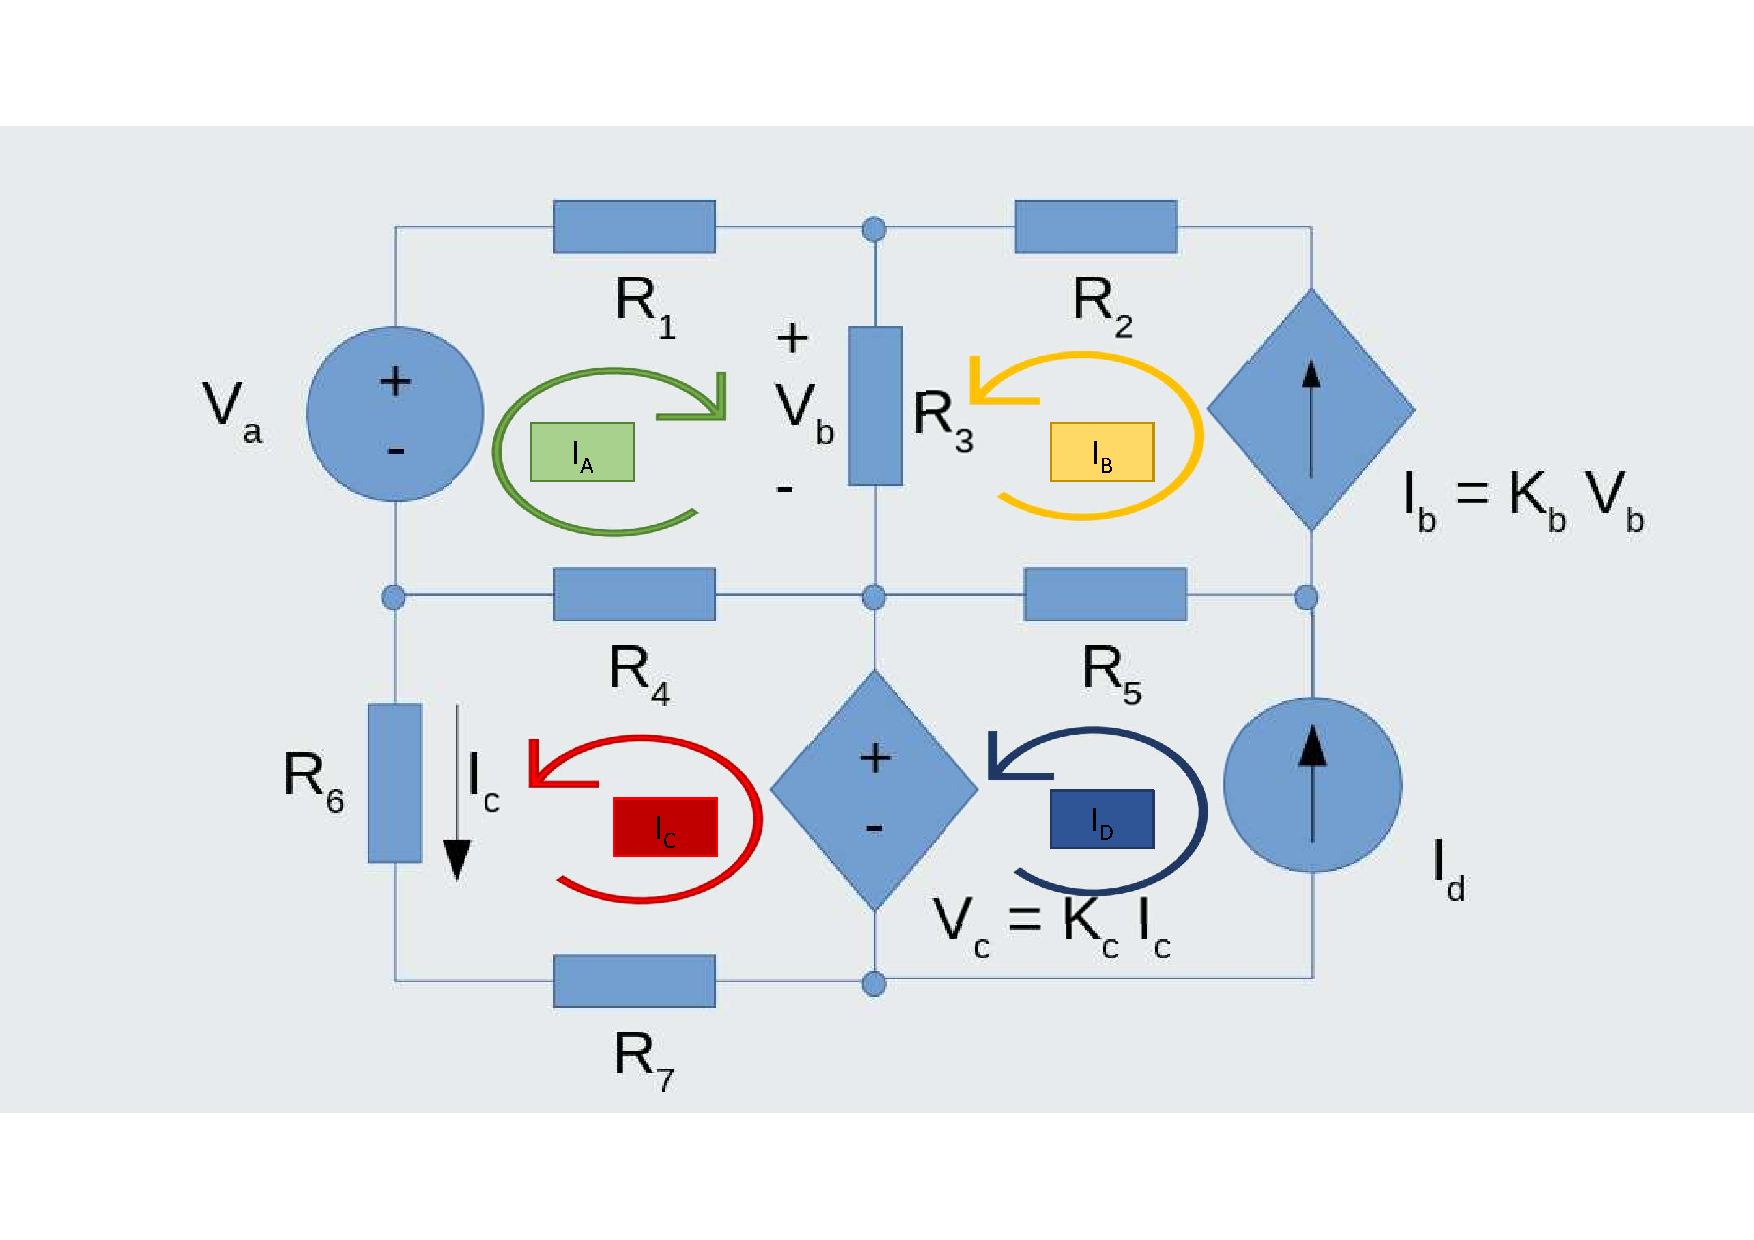
\includegraphics[width=0.8\linewidth]{Images/mesh analysis.pdf}
    \caption{Current flow by mesh.}
    \label{fig:Currents}
\end{figure}


\indent

This circuit is composed by four primary meshes in which we assume the current flows counter-clockwise in every mesh but one, as seen in Figure~\ref{fig:Currents}.

Note that this is merely a convention used in our theoretical computations. The actual physical direction of the current can be obtained by analysing the algebraic sign of the current in each branch. 

To find out the current that flows in each mesh we use the Kirchhoff Voltage Law (KVL) followed by Ohm's Law. 

\begin{equation}
    \sum_{k=1}^{n} V_k = 0.
    \quad\text{,}\quad 
    V=RI.
\end{equation}

In some cases, two currents flow on the same branch. To solve this we use  Kirchhoff Current Law (KCL), to find the current on that branch.

\begin{equation}
    \sum_{k=1}^{n} I_k = 0.
    \label{eq:KCL}
\end{equation}

In mesh $a$ (mesh where the current $I_a$ flows) we assume that the voltage source is providing energy to the circuit and therefore the current has to flow clock-wise. This means that the sum of the voltages in each resistor ($R_1$, $R_3$ and $R_4$) has to equal the voltage $V_a$.

In meshes $b$, $c$ and $d$ we followed the same process as in mesh $a$, defining the way in which the current flows through current and voltage sources.
To exemplify this process, the equation for mesh $a$ is the following:

\begin{equation}
    V_a=R_1I_a+R_3(I_a+I_b)+R_4(I_a+I_c).
\end{equation}

With the aid of octave, we can solve the four equations to obtain the following table (table~\ref{tab:Imesh}).

\begin{table}[h]
  \centering
  \begin{tabular}{|l|r|}
    \hline    
    {\bf Name} & {\bf Value [mA]} \\ \hline
    Ia & 0.194523 \\ \hline 
Ib & -0.204136 \\ \hline 
Ic & 0.961761 \\ \hline 
Id & 0.000000 \\ \hline 

  \end{tabular}
  \caption{Results from the mesh analysis, from \textit{Octave}.}
  \label{tab:Imesh}
\end{table}

Since we know the current on each mesh we can calculate the current on every branch. The results are present on table~\ref{tab:Ibranch}.

\begin{table}[h]
  \centering
  \begin{tabular}{|l|r|}
    \hline    
    {\bf Name} & {\bf Value [mA]} \\ \hline
    Ib & -0.204136 \\ \hline 
Id & 0.000000 \\ \hline 
R1 & 0.194523 \\ \hline 
R2 & -0.204136 \\ \hline 
R3 & -0.009613 \\ \hline 
R4 & 1.156284 \\ \hline 
R5 & 0.204136 \\ \hline 
R6 & 0.961761 \\ \hline 
R7 & 0.961761 \\ \hline 

  \end{tabular}
  \caption{Current on each branch.}
  \label{tab:Ibranch}
\end{table}


\subsection{Node analysis}

\begin{figure}[H] \centering
    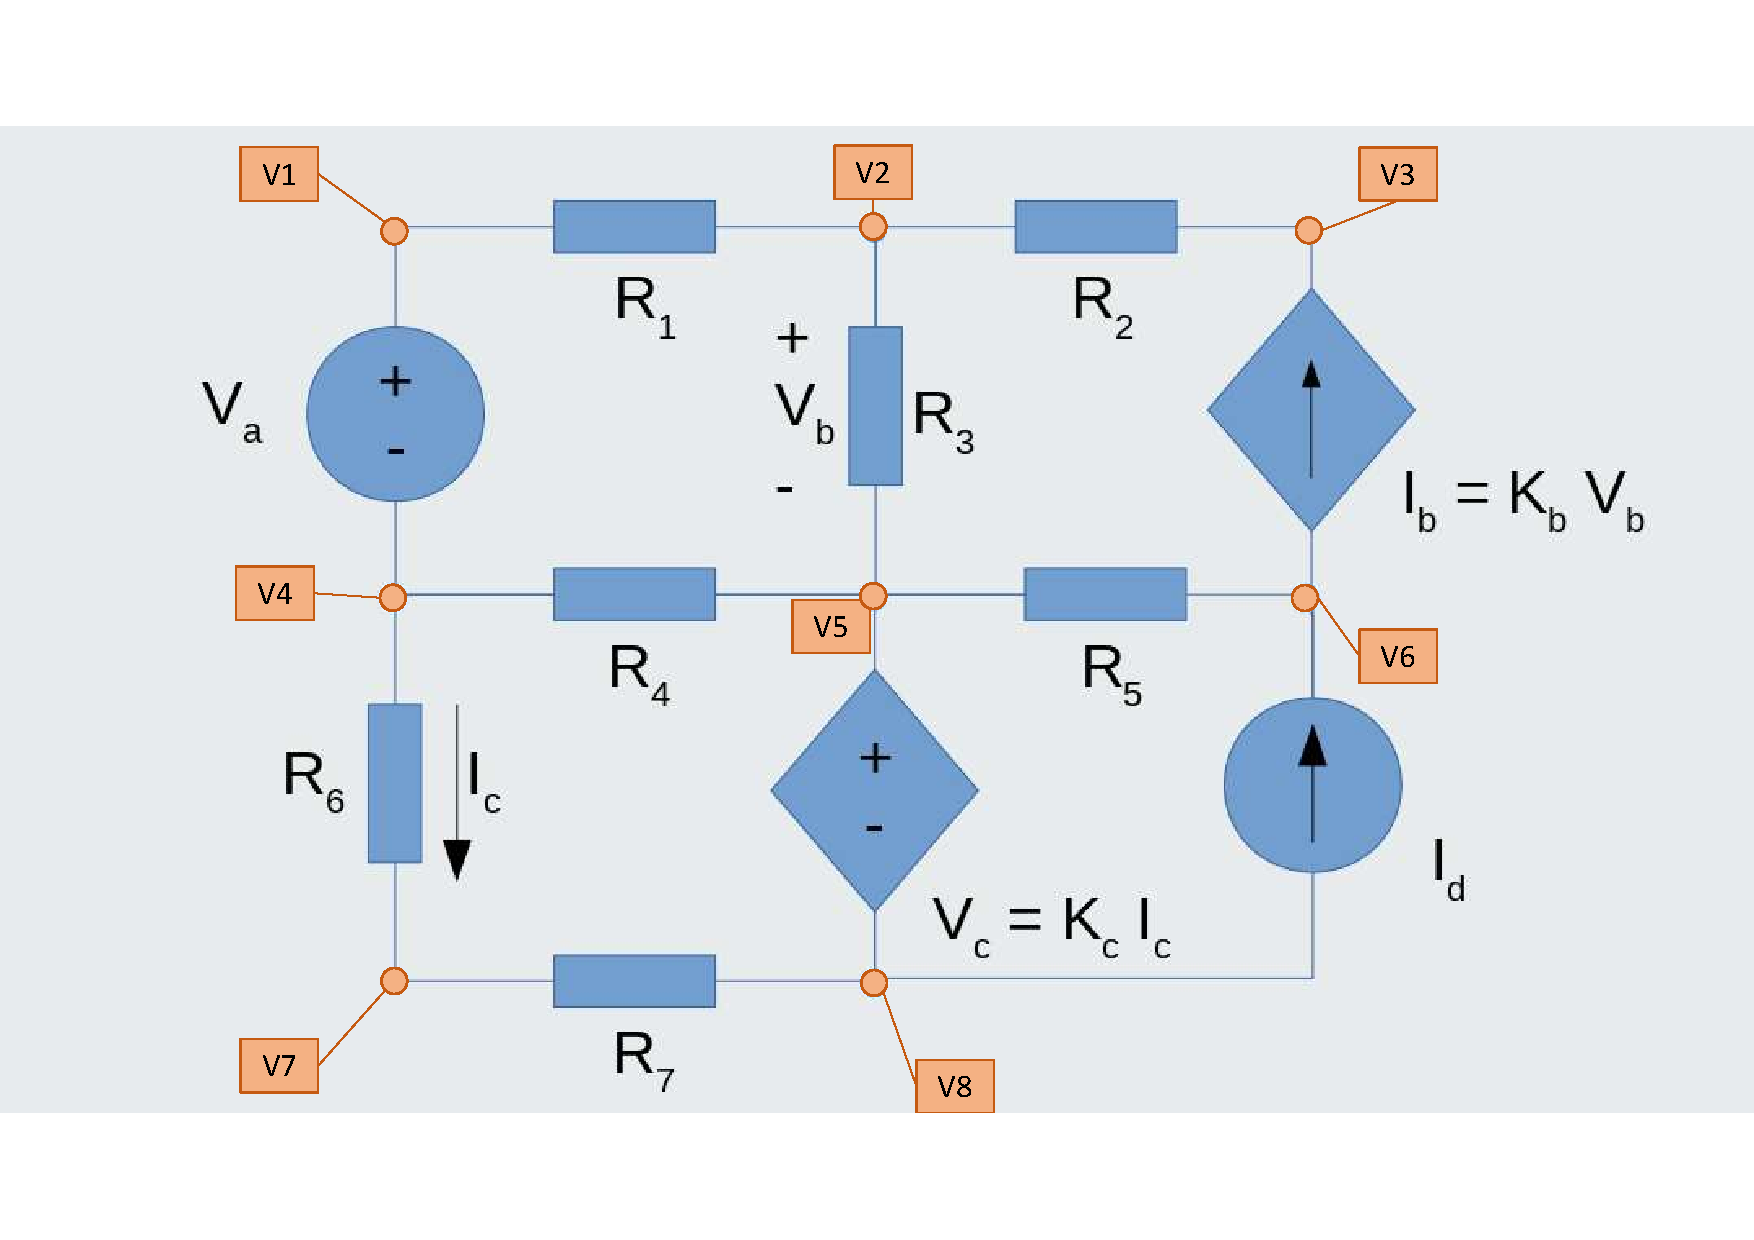
\includegraphics[width=0.8\linewidth]{Images/node analysis.pdf}
    \caption{Nodes.}
    \label{fig:Nodes}
\end{figure}

\indent

There are 8 nodes in total which means that we need 8 equations to find out the voltages in each node and solve the circuit. Therefore, we use the Kirchhoff Current Law (KCL, equation~\ref{eq:KCL}) in every node that is not connected to a voltage source (nodes 2, 3, 6 and 7, which are identified in Figure~\ref{fig:Nodes} ).

We assume node 4 ($V_4$) as the reference node, which means that its value is 0. This node was chosen because usually, the negative terminal of a voltage source is connected to the ground.

It is also known that the value of a voltage source is equivalent to the difference of the voltages in each node to which the source is connected. That allows us to create two more equations, since there are two voltage sources in the circuit.

For the $8^{th}$ equation we can create a supernode with nodes 5 and 8 since the dependent voltage source is not connected to the reference node. This way, nodes 5 and 8 are considered as one by ignoring the voltage source between them.

To demonstrate the process, the node 2 equation resulting from the KCL application is the following:

\begin{equation}
    (V_2-V_3)G_2=(V_5-V_2)G_3+(V_1-V_2)G_1.
\end{equation}

Doing this on all possible nodes/supernode and adding the extra equations, regarding the voltage sources, a system of linear equations can be obtained and solved with the aid of \textit{Octave}. The results are presented on table~\ref{tab:Volts}.

\begin{table}[h]
  \centering
  \begin{tabular}{|l|r|}
    \hline    
    {\bf Name} & {\bf Value [V]} \\ \hline
    V1 & 5.008942 \\ \hline 
V2 & 4.808960 \\ \hline 
V3 & 4.394159 \\ \hline 
V4 & 0.000000 \\ \hline 
V5 & 4.837862 \\ \hline 
V6 & 5.474755 \\ \hline 
V7 & -2.008723 \\ \hline 
V8 & -2.970917 \\ \hline 

  \end{tabular}
  \caption{Results from the node analysis, from \textit{Octave}.}
  \label{tab:Volts}
\end{table}


\pagebreak
\section{Simulation Analysis}
\label{sec:simulation}

\indent

This section discusses the circuit simulation, performed using {\it Ngspice}. 

This circuit was entered into the {\it Ngspice} simulation environment. This tool is used to simulate analog electronic circuits and predict circuit behaviour. 
This {\it Ngspice} simulation begins by defining the ground node, which is the node with potential 0 (by convention). In {\it Ngspice}, the ground node is represented by $V_0$. In our theoretical analysis, the ground node was defined to be node 4. However node 4 is still needed because we must introduce a voltage source with 0V potential, in order to measure the current Ic for the dependent voltage source, since {\it Ngspice} considers the voltage sources as Ammeters.
The new diagram, which represents more accurately what was introduced in {\it Ngspice}, is shown on Figure~\ref{fig:ngspiceCircuit}.

\begin{figure}[h] \centering
    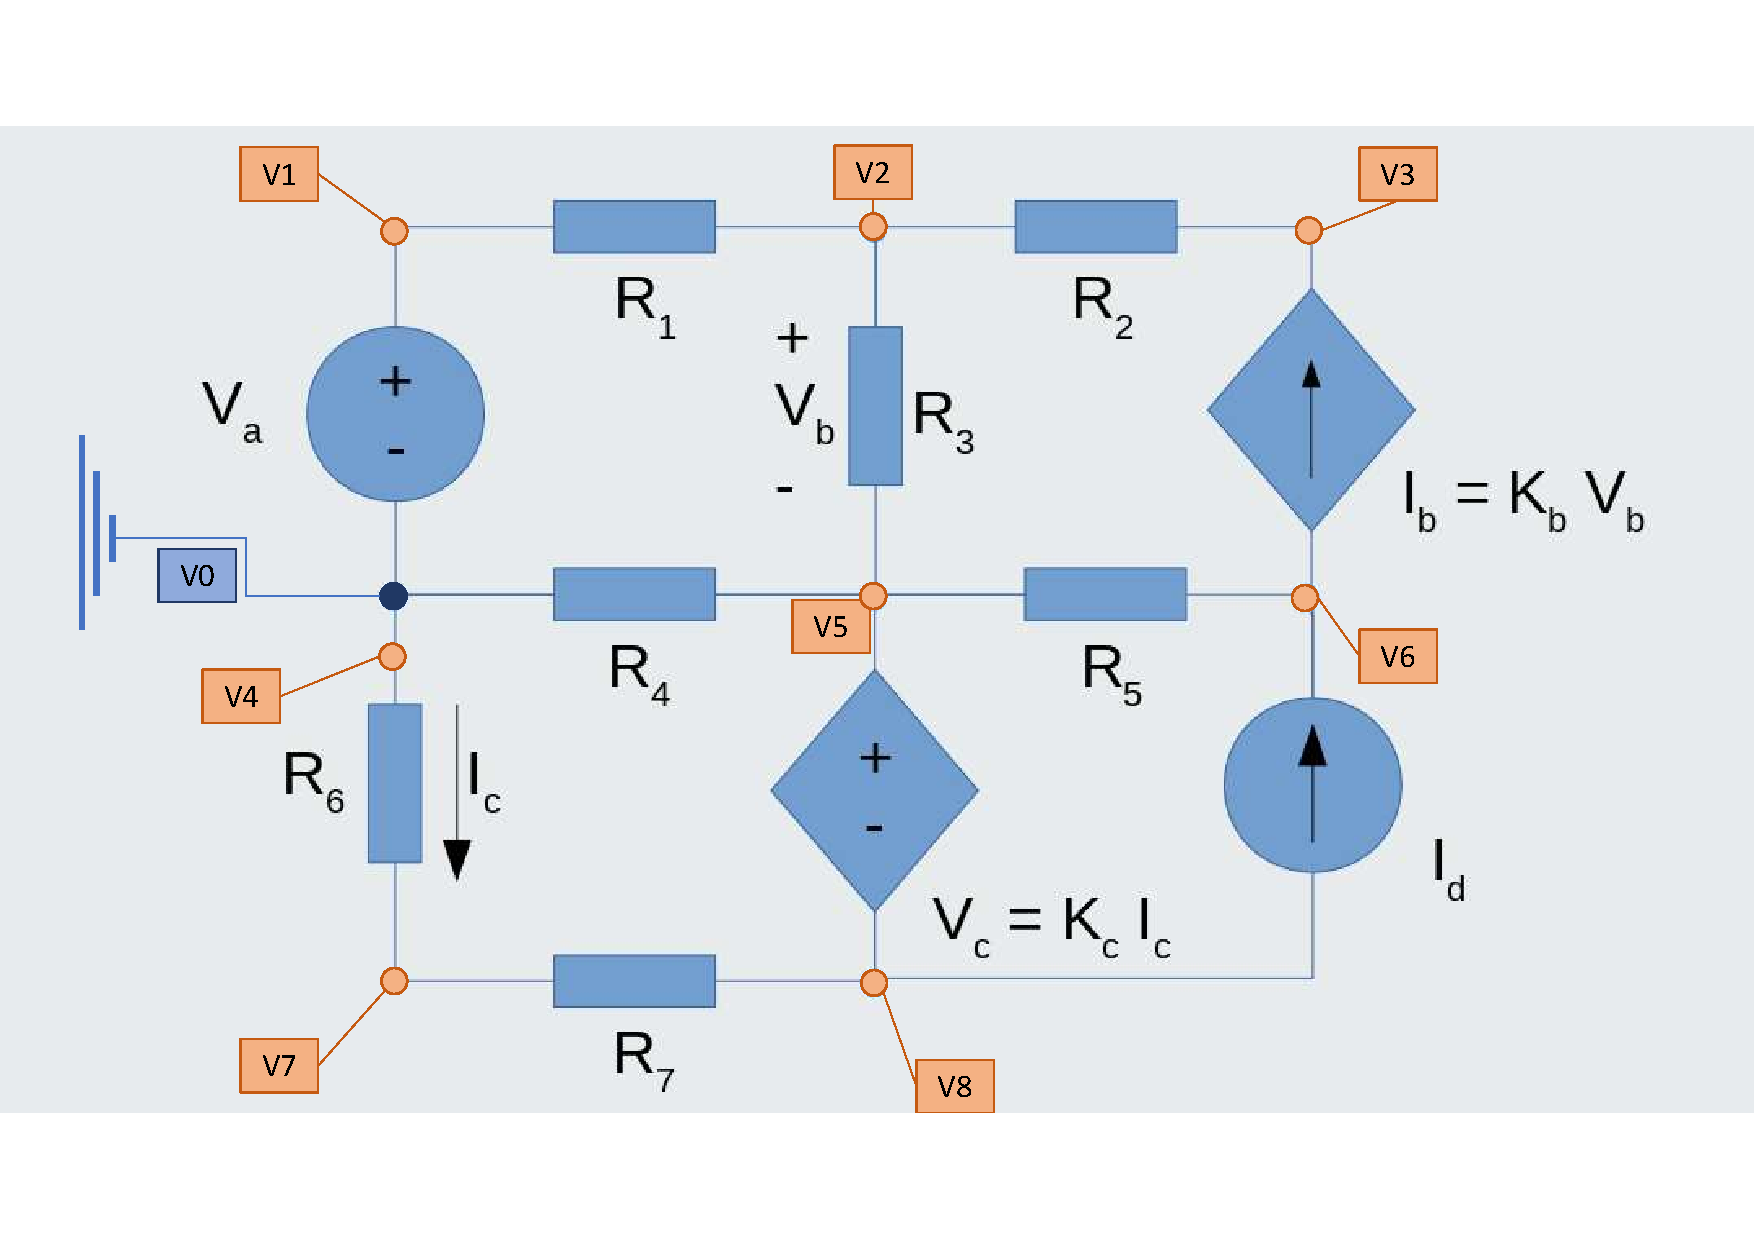
\includegraphics[width=0.8\linewidth]{Images/ngspice model.pdf}
    \caption{Voltage and Current driven circuit with 7 resistors.}
    \label{fig:ngspiceCircuit}
\end{figure}





Table~\ref{tab:op} shows the simulated operating point results for the circuit
under analysis.

\begin{table}[h]
  \centering
  \begin{tabular}{|l|r|}
    \hline    
    {\bf Name} & {\bf Value [A or V]} \\ \hline
    @c[i] & 0.000000e+00\\ \hline
@gcs[i] & -2.04136e-04\\ \hline
@r1[i] & 1.945229e-04\\ \hline
@r2[i] & -2.04136e-04\\ \hline
@r3[i] & -9.61363e-06\\ \hline
@r4[i] & 1.156284e-03\\ \hline
@r5[i] & 2.041365e-04\\ \hline
@r6[i] & 9.617613e-04\\ \hline
@r7[i] & 9.617613e-04\\ \hline
v(1) & 5.008942e+00\\ \hline
v(2) & 4.808960e+00\\ \hline
v(3) & 4.394159e+00\\ \hline
v(4) & 0.000000e+00\\ \hline
v(5) & 4.837862e+00\\ \hline
v(6) & 5.474755e+00\\ \hline
v(7) & -2.00872e+00\\ \hline
v(8) & -2.97092e+00\\ \hline

  \end{tabular}
  \caption{Operating point. A variable preceded by @ is of type {\em current}
    and expressed in Ampere; other variables are of type {\it voltage} and expressed in
    Volt.}
  \label{tab:op}
\end{table}









\pagebreak
\section{Results Analysis}
\label{sec:ResultsAnalysis}

\indent

The simulation results match the predicted ones from the theoretical analysis with precision. This was expected due to the fact that this circuit only contains linear (dependent and independent) components.
%Nevertheless, there are very small differences. This could probably originate from numerical approximation on either {\em Octave} or {\em Ngspice}.


\section{Conclusion}
\label{sec:conclusion}

\indent

In this laboratory assignment, the objective of analysing a circuit with dependent and independent current and voltage sources has been achieved. This circuit has been analysed using the Mesh and the Node methods, which are based on Kirchhoff's Circuit Laws (KVL and KCL, respectively). 

The theoretical equations derived from applying the Mesh and Node methods have been computed and solved using the {\em Octave} Maths tool. These results have then been confronted with the simulation results, which were obtained by using the {\em Ngspice} tool, resulting in a match.

%\cleardoublepage

% ----------------------------------------------------------------------
%  Bibliography
% ----------------------------------------------------------------------
%\addcontentsline{toc}{section}{\bibname}
%\bibliographystyle{abbrvunsrtnat} % <<<<< SELECT IF USING REFERENCES BY NUMBER (CITATION ORDER)
%\bibliography{../../../BIBfile.bib}

% ----------------------------------------------------------------------
\end{document}
% ----------------------------------------------------------------------

